\chapter{Classical and Cloud Computing}
In this chapter we will discuss about classical computing and its limitations compared to quantum computing.
\section{Classical Computing}

The probability of making errors is very high by hand. A computer is a universal machine. A universal machine can be described as an electronic device with the ability to solve problems. These problems have solutions, that can be represented by a set of instructions. These problems are known as computational problems because the classical computer can solve them. 

Computational problems include decision problems, search problems, function problems and optimization problems.  Decision problems are similar to making a choice between true or false, where true can be represented by 1 and false 0. Search problems are like looking for a word in a text. Function problems are for example evaluating $\cos (\theta)$. Optimization problems are problems whereby, you want the output to be the maximum possible value. We therefore find the inputs which satisfy this condition. What prices will you charge the customers in order to make maximum profit without exploiting your customers?

Computers can be connected to each other in order to communicate. This is known as distributed computing. Each processor has its own memory but can communicate with others by sharing messages. One memory can also be shared by multiple processors (parallel computing). Parallelism speeds up computations since different tasks can be performed at the same time. The more the number of processors the more expensive a machine is. 

To solve problems, a computer requires resources. The more resources required the more complex it is described. Thus computational complexity is defined by the resources used. A client may wish to perform tasks which require computational power beyond their capabilities. They may also have limited resources, therefore, they decide to outsource resources from remote servers. The client therefore delegates tasks. Can the client trust the output from the server? If the client cannot trust the server, then this raises a reliability issue. One of the solution to this issue is that, the client can choose multiple servers provided atleast one of them is reliable (honest) and delegate tasks to them \citep{canetti2011practical}. The problem with this protocol is that, it is difficult to determine which server is honest. This makes verifying correctness to be based on probability. This can be done by a client dividing the task into stages. The client can therefore access the output of each stage. This allows the client to check for inconsistencies between the servers' outputs. In case of inconsistencies and if the stage affected can easily be performed by the client, then determining the dishonest server becomes simple otherwise it would be very difficult. There are times when a client requires urgent results. During these times, the client may have no time to compare outputs from different servers. Requiring services from different servers is expensive and time consuming.

Servers could decide to give false results (dishonest) based on a couple of reasons. The resources required to perform the computation may be a lot to the server. This makes the profit made less than the estimated one. The server could also benefit from some outputs for example poll results. An employee could just decide to interfere with the computations being executed \citep{canetti2011practical}. 


Cloud computing is an example of a delegated computing system.


\section{Cloud Computing}
\subsection{What is Cloud Computing?}
Cloud Computing is the process whereby, computation is done somewhere else (in the cloud), and is similar to working on your personal computers \citep{hayes2008cloud}. Cloud is some server stored somewhere anonymous only the service providers knows about its whereabouts. Clients for example companies or individuals are able to request services such as storage, manipulation of data and computations among others. Cloud services are offered as demanded by the clients. Clients do not have to train their staff, worry about data loss in case of system crashes, buy new infrastructure or get licenses for softwares.

The three major types of cloud computing services are: Platform as a Service (PaaS) such as Google App Engine (which is mainly used by developers), Software as a Service (SaaS) for example email and Facebook and Infrastructure as a Service (IaaS) like storage facilities and servers.

Examples of companies offering cloud services include Amazon, Google and IBM.

The main disadvantage of cloud computing is security on \citep{subashini2011survey} and \citep{miller2008cloud}. 
Security is one of the issues that is making some companies to shy away from cloud computing. Most governments have rules that their sensitive information should not leave their respective countries. The cloud servers may be located anywhere in the world. In cloud computing data may be changed and this interferes with its integrity. Integrity can be defined as the quality of wholeness. Data which has been changed is not whole. Data could be changed to manipulate intended results. Duplication of data could also occur. This amounts to information theft. In cloud computing making an exact copy of data is possible and the client may not learn about it in good time. Data can be interfered with. Since many clients are using the same server, the possibility of their data mixing up is very high. Some clients could also be malicious and interfere with other client's data. Leakage may also occur. Sensitive information may be exposed to unintended audience. For example, if a user receives emails from different people but always performs a search on a specific sender, this could reveal to the server that this person has a level of importance to the client. The server may exploit this loophole to gather information on why this person interest the client.

The bottom line is, we do not trust the server. Our privacy, confidentiality and integrity is put at risk. The data may end up falling into the wrong hands with unauthorized personnel which would lead to severe consequences. Organizations whose data is mainly sensitive information, would find it hard to adopt cloud computing. A user can encrypt data before storing it in the cloud and when he/she needs it they can download and decrypt it. Thus, this user cannot use other services apart from the storage. Other costs of hardware and software, which will be used to process the data are incurred \citep{yang2013evaluation}.

A solution to this is homomorphic encryption, whereby a server performs computations on encrypted data.

\section{Classical Homomorphic Encryption and its Limitations}
Homomorphic Encryption is also an example of a delegated computing system. This system ensures secure delivery of information, storage and computations. Homomorphic encryption is the ability of a server to work on encrypted data. According to \citet{ogburn2013homomorphic}, homomorphic encryption can either be partial, somewhat or fully. In Partial Homomorphic Encryption, you can either perform addition or multiplication on encrypted data but not both. A Somewhat Homomorphic Encryption technique has the ability to perform both multiplication and addition on limited numbers. A Fully Homomorphic Encryption can support both multiplication and addition and is not limited to any numbers. Most of us would choose a Fully Homomorphic Encryption system. Its only disadvantage is that, it is less efficient as compared to Partial Homomorphic Encryption and Somewhat Homomorphic Encryption. 

Figure \ref{fig1 : Encrypt} is an example of a Homomorphic Encryption. The words are concatenated after encryption. The result obtained after decryption, is the same with the result if the concatenation was performed without the encryption.
\begin{figure}[!h]
\center
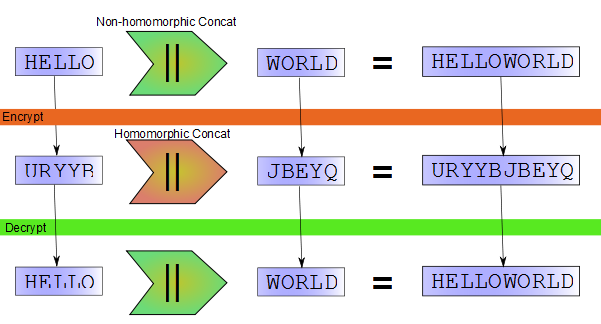
\includegraphics[scale= 0.5]{images/encrypt.png} 
\caption{Encrypted concatenation}
\label{fig1 : Encrypt}
\citep{Craig}
\end{figure}

\subsection{Why is Homomorphic Encryption considered secure?}
As it can be seen from Fig \ref{fig1 : Encrypt}, no information is revealed to the server. The server can learn about the information only if it can decrypt it. The server can only decrypt the information if they know how you as the client encrypted it and they possess the decryption key. This may be termed as negligence from the client's side. In Homomorphic Encryption the integrity of the data is maintained. How will the server change something like 'JBEYQ' which they can't even interpret? The client may get some results and tell that something is wrong, in case the server changes something. It is very easy to manipulate something that you can understand but difficult otherwise. Data cannot be duplicated. The encrypted data can be duplicated but the real unencrypted data cannot. Sensitive information cannot leak too. Privacy and secrecy are also maintained.

\subsection{Limitations of Classical Homomorphic Encryption as compared to Quantum Homomorphic Encryption}
We always seek to improve the existing things. The big question is why Quantum and not Classical?	A classical computer is limited in terms of computation power as compared to a quantum computer. Some tasks like factorization that can be performed easily on a quantum computer are hard and require a lot of time on a classical computer \citep{unruh1995maintaining}. The main idea is to improve speed and efficiency. This is especially when dealing with large chunks of data like performing a search operation in a large database and factorization of large numbers. 

This makes Quantum Homomorphic Encryption attractive. 

%First of no information about the data is revealed unless the server can decrypt it.
